%%%%%%%%%%%%%%%%%%%%%%%%%%%%%%%%%%%%%%%%%
% Beamer Presentation
% LaTeX Template
% Version 1.0 (10/11/12)
%
% This template has been downloaded from:
% http://www.LaTeXTemplates.com
%
% License:
% CC BY-NC-SA 3.0 (http://creativecommons.org/licenses/by-nc-sa/3.0/)
%
%%%%%%%%%%%%%%%%%%%%%%%%%%%%%%%%%%%%%%%%%

%----------------------------------------------------------------------------------------
%	PACKAGES AND THEMES
%----------------------------------------------------------------------------------------
\documentclass{beamer}

\mode<presentation> {

% The Beamer class comes with a number of default slide themes
% which change the colors and layouts of slides. Below this is a list
% of all the themes, uncomment each in turn to see what they look like.

%\usetheme{default}
%\usetheme{AnnArbor}
%\usetheme{Antibes}
%\usetheme{Bergen}
%\usetheme{Berkeley}
%\usetheme{Berlin}
%\usetheme{Boadilla}
%\usetheme{CambridgeUS}
%\usetheme{Copenhagen}
%\usetheme{Darmstadt}
%\usetheme{Dresden}
%\usetheme{Frankfurt}
%\usetheme{Goettingen}
%\usetheme{Hannover}
%\usetheme{Ilmenau}
%\usetheme{JuanLesPins}
%\usetheme{Luebeck}
\usetheme{Madrid}
%\usetheme{Malmoe}
%\usetheme{Marburg}
%\usetheme{Montpellier}
%\usetheme{PaloAlto}
%\usetheme{Pittsburgh}
%\usetheme{Rochester}
%\usetheme{Singapore}
%\usetheme{Szeged}
%\usetheme{Warsaw}

% As well as themes, the Beamer class has a number of color themes
% for any slide theme. Uncomment each of these in turn to see how it
% changes the colors of your current slide theme.

%\usecolortheme{albatross}
%\usecolortheme{beaver}
%\usecolortheme{beetle}
%\usecolortheme{crane}
%\usecolortheme{dolphin}
%\usecolortheme{dove}
%\usecolortheme{fly}
%\usecolortheme{lily}
%\usecolortheme{orchid}
%\usecolortheme{rose}
%\usecolortheme{seagull}
%\usecolortheme{seahorse}
%\usecolortheme{whale}
%\usecolortheme{wolverine}

%\setbeamertemplate{footline} % To remove the footer line in all slides uncomment this line
%\setbeamertemplate{footline}[page number] % To replace the footer line in all slides with a simple slide count uncomment this line

%\setbeamertemplate{navigation symbols}{} % To remove the navigation symbols from the bottom of all slides uncomment this line
}
%----------------------------------------------------------------------------------------
\usepackage{graphicx} % Allows including images
\usepackage{booktabs} % Allows the use of \toprule, \midrule and \bottomrule in tables
\usepackage{subfigure}
\setbeamerfont{caption}{size=\scriptsize}
\usepackage{hyperref}
\usepackage{listings}
%----------------------------------------------------------------------------------------
%	TITLE PAGE
%----------------------------------------------------------------------------------------
\title[]{ROS Tools: rqt} % The short title appears at the bottom of every slide, the full title is only on the title page
%----------------------------------------------------------------------------------------
\author{ARRA / AR2A} % Your name
\institute % Your institution as it will appear on the bottom of every slide, may be shorthand to save space
{
\textbf{A}dvancements for \textbf{R}obotics in \textbf{R}escue \textbf{A}pplications
}
\date{\today} % Date, can be changed to a custom date
%----------------------------------------------------------------------------------------
\begin{document}
%----------------------------------------------------------------------------------------
\begin{frame}
\titlepage % Print the title page as the first slide
\end{frame}
%----------------------------------------------------------------------------------------
%	PRESENTATION SLIDES
%----------------------------------------------------------------------------------------
\begin{frame}{ARRA/AR2A}
\begin{large}\textbf{What do we want?}\end{large}
\begin{itemize}
 \item ARRA / AR2A aims to improve the current state of technology of robotics in rescue applications.
\end{itemize}
\begin{large}\textbf{Who are we?}\end{large}
\begin{itemize}
 \item A volunteer non-profit organisation of robotic enthusiasts.
\end{itemize}
\begin{large}\textbf{How can you help?}\end{large}
\begin{itemize}
 \item Check us out at \url{https://github.com/ar2a}
\end{itemize}
 \vspace{1cm}
\begin{large}\textbf{License information}\end{large}
\begin{itemize}
 \item \textbf{CC-BY-SA 4.0} \url{https://creativecommons.org/licenses/by-sa/4.0/}
\end{itemize}
\end{frame}
%----------------------------------------------------------------------------------------
\begin{frame}{Overview}
\begin{itemize}
 \item 	\textbf{rqt} is a software framework of ROS that implements the various GUI tools in the form of plugins.
\end{itemize}
\begin{itemize}
 \item One can run all the existing GUI tools as dockable windows within rqt!
\end{itemize}
\begin{itemize}
 \item There are different opportunities to debug with rqt plugins. For example with the \textbf{Console} plugin under \textbf{Plugins/Logging} displays messages as seen in example 1 and 2.
\end{itemize}
\end{frame}
%----------------------------------------------------------------------------------------
\begin{frame}{rqt Example 1}
\begin{figure}[p]
	\centering
	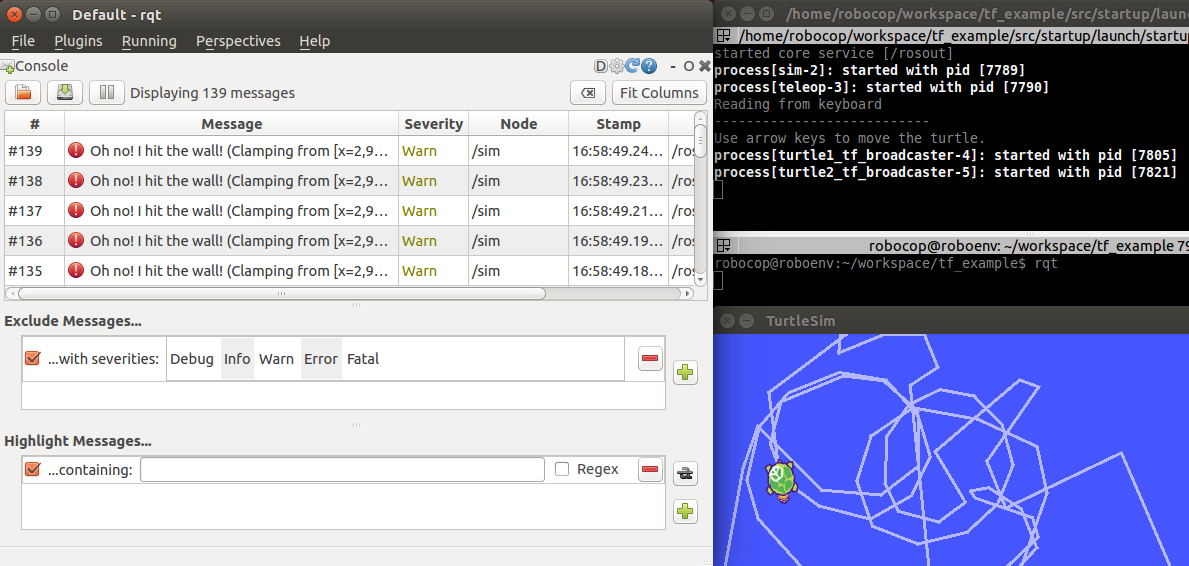
\includegraphics[width=1\textwidth]{./images/rqt.png}
	\caption{Read messages with rqt turtle demo.}
	\label{fig::rqt_1}
\end{figure}
\end{frame}
%----------------------------------------------------------------------------------------
\begin{frame}{rqt Example 2}
	\begin{figure}[p]
		\centering
		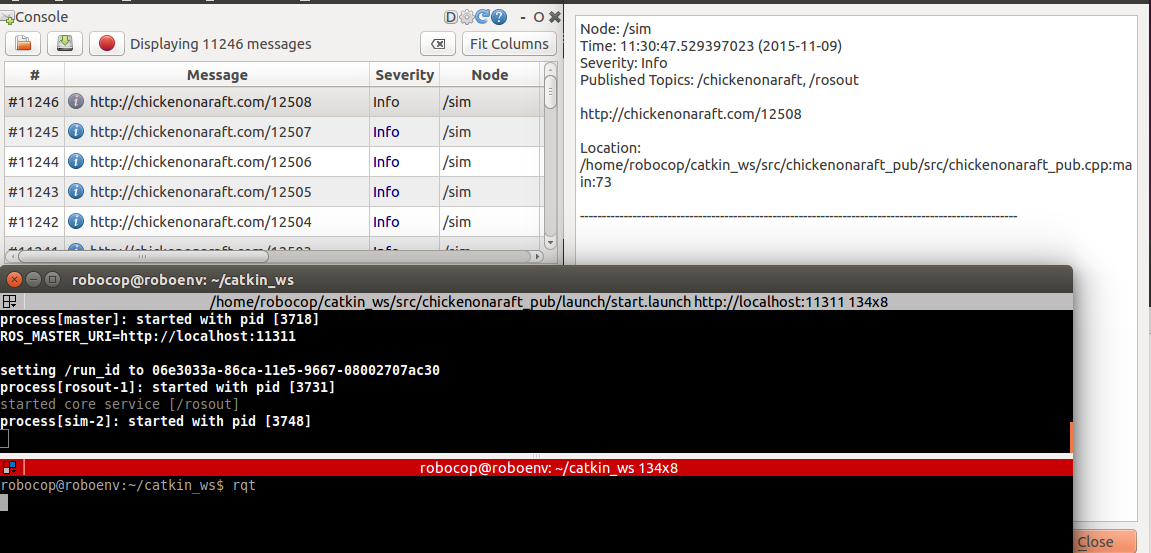
\includegraphics[width=1\textwidth]{./images/chickenrqt.png}
		\caption{Read messages with rqt from chicken demo.}
		\label{fig::rqt_2}
	\end{figure}
\end{frame}
%----------------------------------------------------------------------------------------
\begin{frame}
\Huge{\centerline{The End}}
\end{frame}
%----------------------------------------------------------------------------------------
\end{document} 
%----------------------------------------------------------------------------------------